\subsection{Project characteristics}
% Charakterystyka projektu i sposób jego realizacji - macie tutaj napisać co to był za projekt (badawczy, rozwojowy) a wiec czy wymagania były jasne czy tak naprawdę powstawały w jego trakcie. Ważne by spróbować scharakteryzować przyjęty sposób realizacji a wiec przyjęty proces np. czy to był proces przyrostowy czy iteracyjny. Najczęściej Wasz proces jest oparty na prototypowaniu z odrzucaniem przez pierwszy semestr, a potem to typowy proces przyrostowo-iteracyjny w drugim semestrze. Spróbujcie napisać również z czego to wynika.

Our projects is special for a few reasons.

First of all, we came up with a project idea ourselves and tried to find a person that would be interested in being a thesis supervisor.
Taking that into account, the requirements for the project were not defined beforehand
and we learned more and more about them as the project developed.
Due to that fact, it was both easier and harder for us to do our job as architects and developers.
On the one hand, it was mostly us who were responsible for the direction the project would take, but at the same time, at each step of the process
we had to struggle with choosing which parts of the project would be more attractive for our client, our future users, and from the scientific point of view.

Second of all, some of the problems we were faced with come from the field of \textit{Computational Origami}.
It's a relatively new branch of science, which ideas span the realms of mathematics, physics, 
computer science, engineering, and even architecture.
Also, it is not a subject that would normally be taught during one's educational career.
Of much help to us was Prof. Erik Demaine and his MIT course on Geometric Folding Algorithms: Linkages, Origami, Polyhedra \cite{mit-course}
\smallskip

Taking into consideration all the facts mentioned above, our work did not have a specifically structured approach.
We were working in a very simplified \textbf{Kanban} method, where we would select things to work on
as the project unfolded. 
\smallskip

For the better part of the first semester,
we were creating a prototype that would serve as a \textit{Minimal Valuable Product}.
Later on, we did not discard it altogether, but started adding more features on top of it,
polishing it and refactoring when necessary. 
We continued with this approach till the end.

\subsection{Team}
% Osoby w projekcie - często projekt jest robiony dla kogoś a opiekun ma jakieś osoby pomocnicze. Wskażcie wszystkie osoby i ich role w projekcie. Bardzo ważny punkt z formalnego widzenia projektu, gdyż każda osoba musi zostać oceniona w sposób indywidualny.

Our team consisted of our thesis supervisor and us.

\begin{enumerate}
	\item \textbf{Witold Alda} - thesis supervisor.
	\item \textbf{Maciej Mionskowski} - developer, architect.
	\item \textbf{Antoni Mleczko} - developer, architect.
\end{enumerate}

\subsection{Responsibilities in the team}
% Zespól i podział obowiązków - musicie napisać co kto robił. Jeśli wszystko robiliście razem to spróbujcie wskazać chociaż 2-3 główne zadania, którymi każde z Was się zajmowało.

Although we were distributing workload equally between the team members
and each of us touched on all parts of the project, some areas 
received more attention from one person than the other.
To be able to define how much of a percentage each one of us has contributed to the 
given area of the project, first we need to define those areas.
\smallskip

Project areas:
\begin{itemize}
	\item Solver backend
	\item Frontend
	\item Community backend
	\item DevOps / Infrastructure
	\item Thesis
	\item Research
	\item Requirements formulation
\end{itemize}

Having defined project areas, we have agreed upon how much of a contribution each of
us has provided to the given area.

\begin{figure}[H]
  \caption{Maciej's percentage contribution to the areas of the project.}
  \centering
  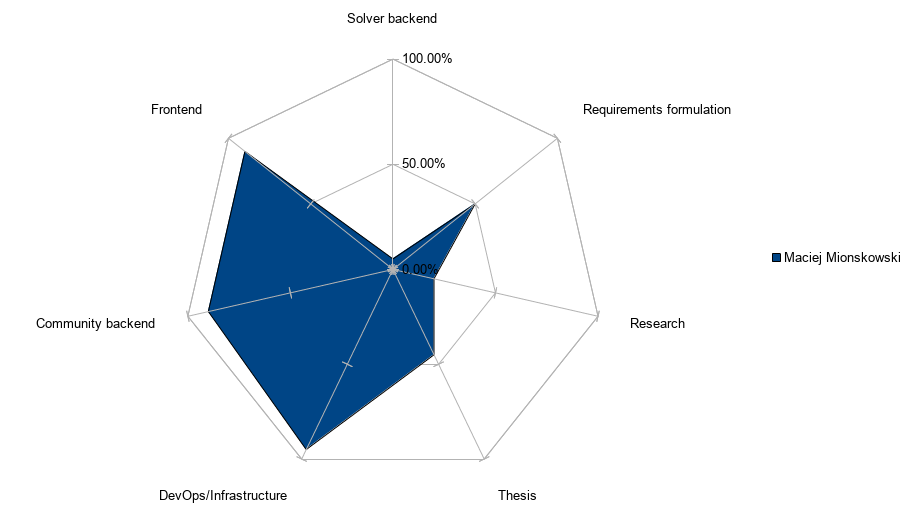
\includegraphics[width=\textwidth]{assets/4-percentage-maciej.png}
\end{figure}

\begin{figure}[H]
  \caption{Antoni's percentage contribution to the areas of the project.}
  \centering
  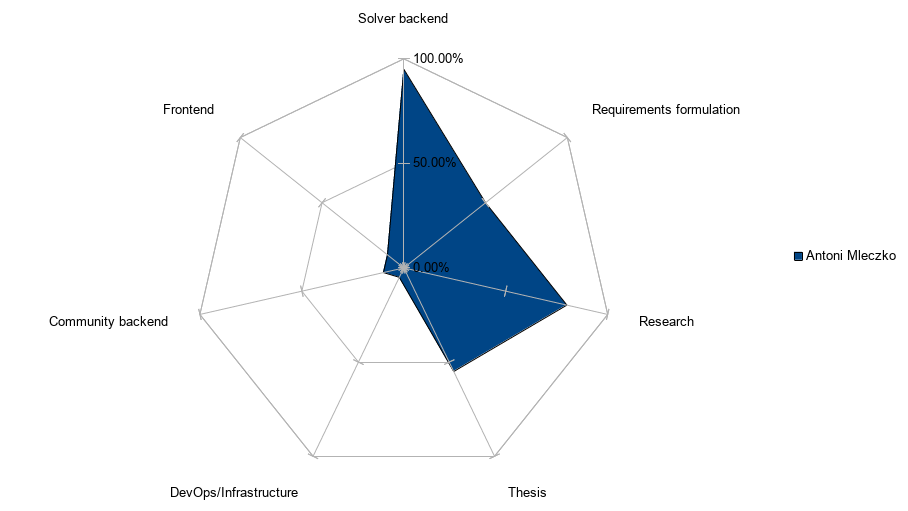
\includegraphics[width=\textwidth]{assets/4-percentage-antoni.png}
\end{figure}




\subsection{Organization of work}
% Organizacja prac i wykorzystane narzędzia - używaliście facebooka, emaili czy spotykaliście się zawsze o określonej porze? Jak i kiedy dzieliliście się zadaniami: czy było to po każdym spotkaniu z klientem? Kiedy spotykaliście się z klientem? Jak często? Używaliście Jiry, confluence, trello? Koniecznie zróbcie screenshota! A może jakieś statystyki z githuba które jakoś podsumują Wasz projekt? Tutaj Wasze przemyślenia i komentarze mile widziane.
% Zastosowane techniki i praktyki - odnosi się do powyższego, ale możecie tutaj spróbować wskazać takie praktyki jak Pair Programming, TDD, Refactoring, Planning Game, User Stories, Team Velocity, Continuous Integration, Sprint Review Meeting, makiety GUI. Jak wyglądał proces testowania? Czy były robione jakieś prototypy? Jak były walidowane, odrzucane (te kwestie ew. do dokumentacji technicznej)?

\subsubsection{Tools}

\tech{Github} was our provider of choice for hosting the code repository, planning work, incorporating continuous integration, continuous delivery, and tracking progress. Despite some of the project management  and CI related features on Github being relatively new and simple, they were suitable enough for our needs. Using the same service for managing all project aspects allows for natural cross-referencing between issues and code. It also acts as a single source of truth, hence reducing the hassle associated with jumping between platforms and keeping them synchronized. 

For creating diagrams we used \tech{diagrams.net} (formerly draw.io), \tech{canva.com}, and \tech{TikZ}. \tech{GIMP} was used for editing screenshots and graphics. System mock-ups were designed in \tech{Adobe XD}.

\subsubsection{Work methodology}

Our work methodology was simple, agile, and based on the Kanban system.

\medskip
We used multiple Github project boards to incorporate Kanban into our environment. 
Community Backend, Solver Backend, Thesis, and Infrastructure each received their separate Kanban Boards. Every Board could represent a separate team working on the project.

\begin{figure}[H]
  \caption{One of the many Kanban Boards in our project.}
  \centering
  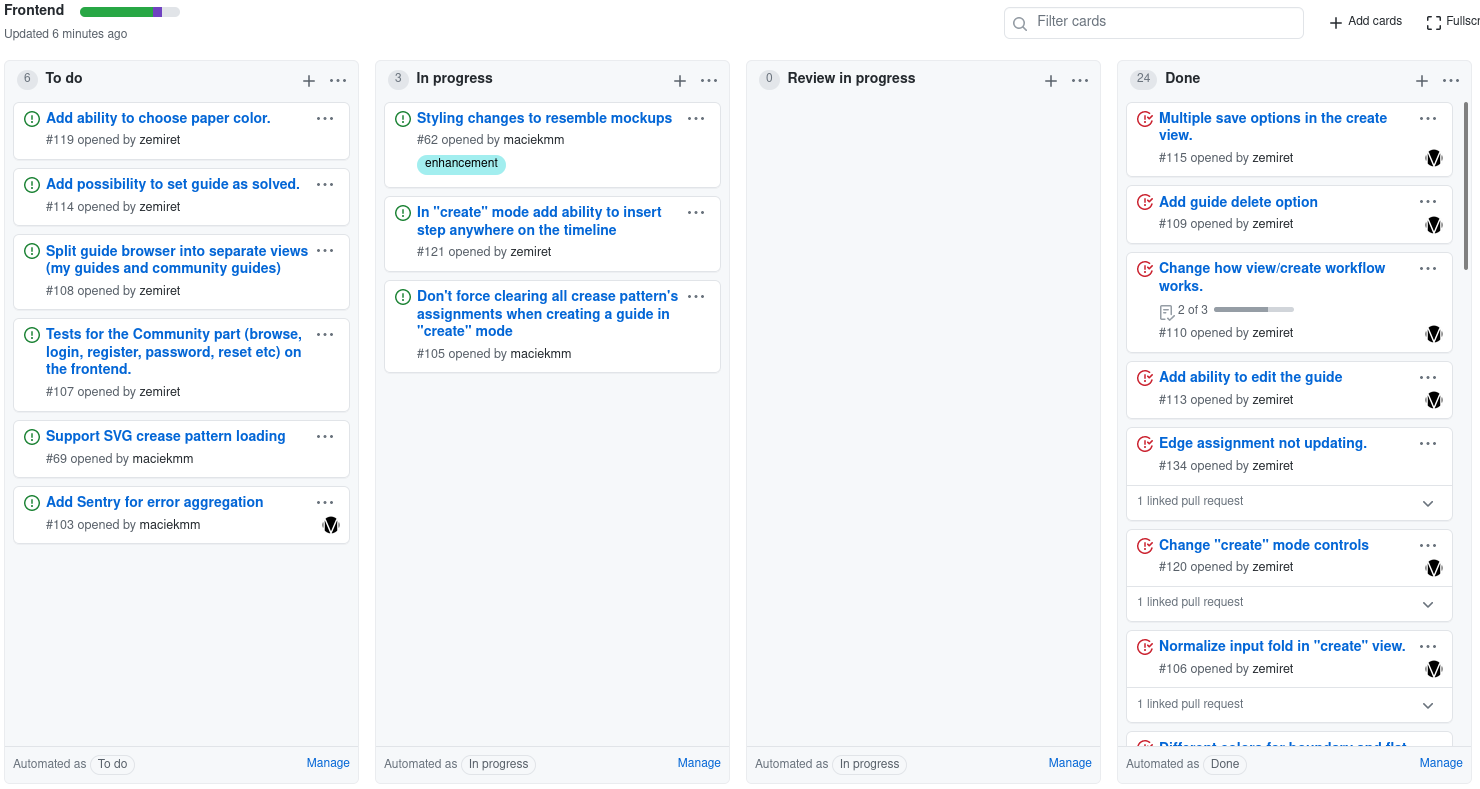
\includegraphics[width=\textwidth]{assets/4-gh-board.png}
\end{figure}

We would pick issues to work on by moving a card from the \textbf{To Do} to the \textbf{In progress} column. Once the development was finished and ready for a review, a Pull Request would be created and the card would be marked as \textbf{Review in progress}. Should a feature pass the review process, the card would be moved to the \textbf{Done} lane.

\medskip 

After we established all functional requirements, they acted as our guide for creating issues. Feature's priority impacted the position of the card in the \textbf{To Do} column. The more important the feature was, the higher it appeared on the \textbf{To Do} pane.

\subsubsection{Communication}

\textbf{Internal}

Thanks to all development team members working from the same place, most of the communication was carried out face to face. This fact had a positive impact on the project as ideas were communicated clearly and quickly. Non-urgent matters were handled through Github issues.

\medskip

\textbf{External}

E-mail was used as the main mean of information exchange between the developer team and the thesis supervisor. Occasionally, phone calls and \tech{Microsoft Teams} were used when a longer discussion was needed. The communication was established primarily in situations when we wanted to confirm a path the project is heading.


\subsubsection{Code development}

As a version control framework we used a simplified \tech{Git workflow}. Each feature would be first developed on a feature branch. Once the work was finished, a Pull Request would be created. The Pipeline would run tests against the changed components. Should the pipeline pass, the review process would commence. Once the work was successfully reviewed, the \texttt{master} branch would be rebased onto the feature branch to avoid merge conflicts. The Pull Request would then be squashed and merged into the \texttt{master} branch. The main branch would run the Pipeline with an additional delivery step, which would result in the code being published to the production environment.




\subsection{Project timeline}
% Przebieg prac (harmonogram, kalendarz): podział na poszczególne etapy, iteracje i jak one wyglądały i co było ich efektem.

The idea for the project was born in Februrary 2020, during a brainstorming session.
The project began in March 2020 and was finalized in December 2020.

\medskip

The general overview of the project timeline can be presented in four phases:
\begin{enumerate}
	\item \textbf{Brainstorming}, during which we held a couple of brainstorming sessions and came up with a few dozen of project ideas.
	\item \textbf{Idea Formalization}, in the midst of which we looked for a supervisor.
	\item \textbf{Topic Research}, throughout which we gathered required scientific knowledge.
	\item \textbf{Development}, during which we developed an actual product.
\end{enumerate}

The diagram below depicts the estimated phase lengths during the project time frame.

\begin{figure}[H]
\label{4-project-phases}
  \caption{Project phases timeline}
  \centering
    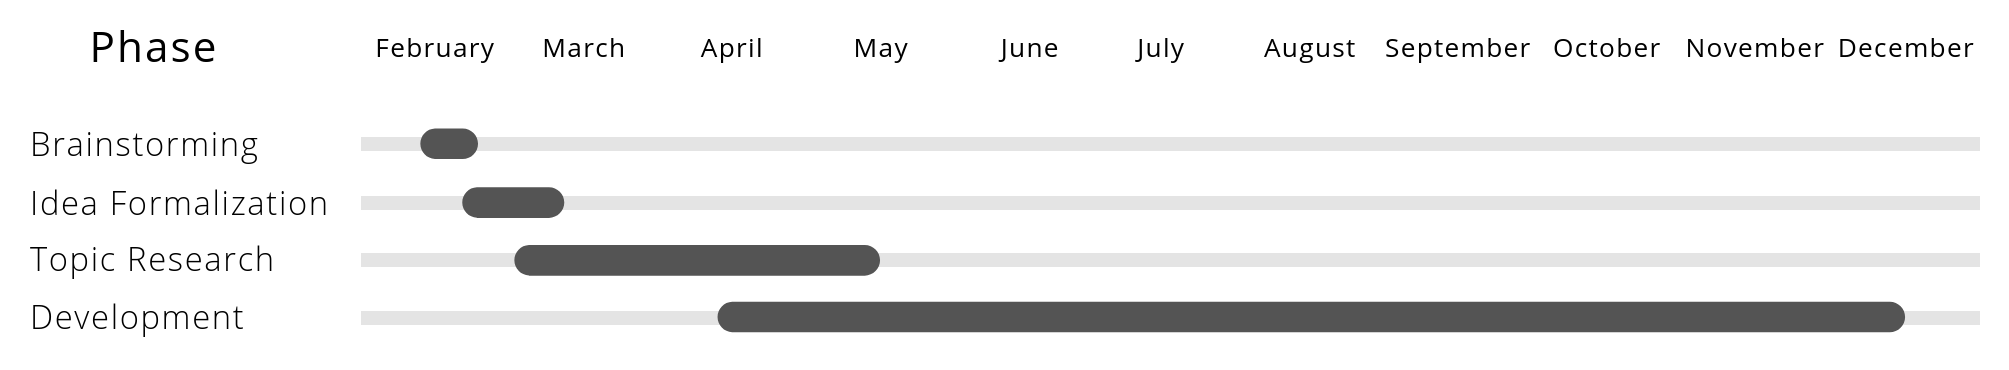
\includegraphics[width=\textwidth]{assets/4-phases.png}
\end{figure}

To see how different aspects of the project unfolded, a more detailed graphic has been created. The data has been mostly sourced from the project's code repository.

\begin{figure}[H]
	\label{04-component-timeline}
	\caption{Components development timeline}
  	\centering
    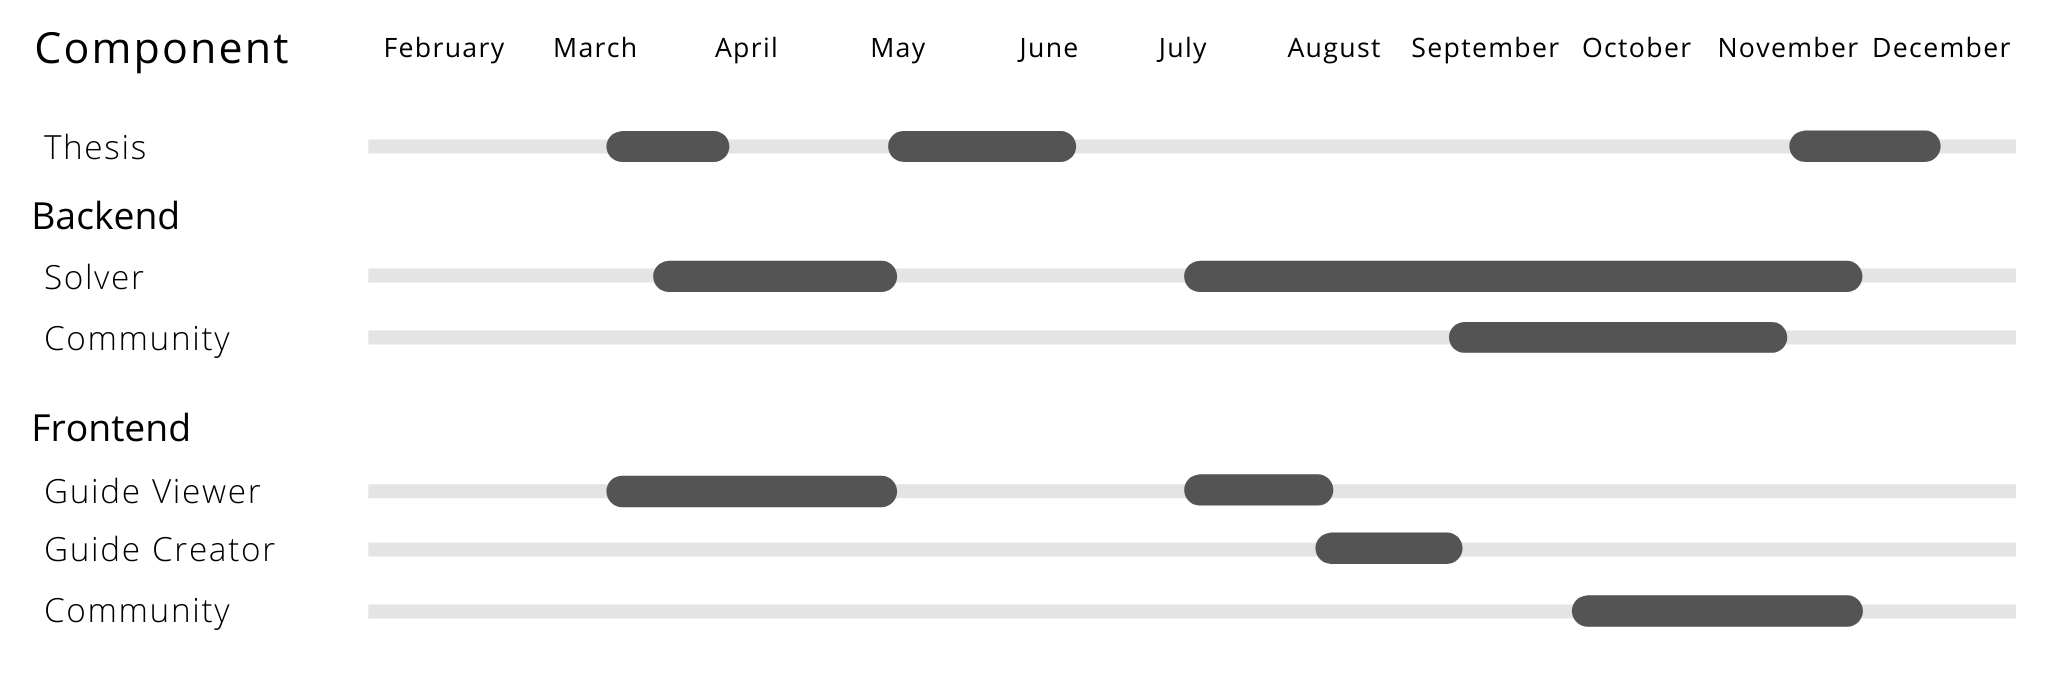
\includegraphics[width=1.01\textwidth]{assets/4-component-timeline.png}
\end{figure}

As can be seen, the work has been pretty well planned and thought out. The actual development time spans the whole project time frame.

The figure below presents the estimated intensity of work.

\begin{figure}[H]
	\label{04-commit-intensity}
	\caption{The project contributions graph - the number of commits to the \texttt{master} branch.}
  \centering
    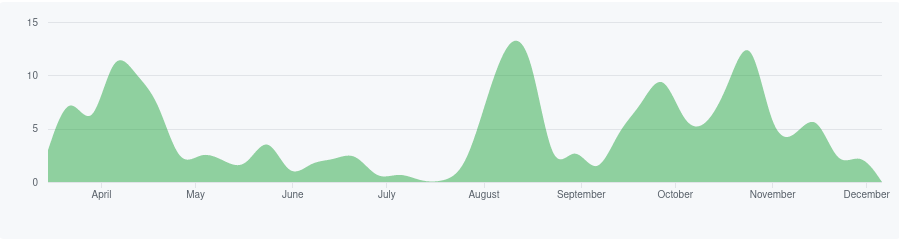
\includegraphics[width=1.01\textwidth]{assets/4-contributions-graph.png}
\end{figure}

The more detailed monthly breakdown of the project state, with features on which we worked, is listed below.

\subsubsection{March}

At the beginning of March we were looking for a supervisor, formulating problems, and planning the project.

\medskip

Having all the formal issues sorted out, we started the Topic Research phase.

Most of the time was spent on studying the \textit{Geometric folding algorithms: Linkages, Origami, Polyhedra} course\cite{mit-course}. The videos provided us with knowledge concerning the scientific field of computational origami, and most importantly:
\begin{itemize}
	\item the terminology,
	\item current numerical algorithms for paper solving problems,
	\item on-going research,
	\item a file format for saving crease patterns,
	\item pitfalls to avoid.
\end{itemize}

It is hard to imagine this project coming to fruition without getting familiar with the aforementioned course.

\subsubsection{April}

April was the start of the Development phase.

We started prototyping, in parallel, the following components:
\begin{itemize}
	\item the Guide Viewer
	\item the Solver.
\end{itemize}

Most notable features that were completed in April include:
\begin{itemize}
	\item adapting the \tech{.fold} file specification to suit the project needs,
	\item \tech{.fold} file parsing on both the backend and the frontend,
	\item \tech{.fold} file rendering on the frontend,
	\item the frontend deployment pipeline,
	\item triangulation on the backend.
\end{itemize}
The end of April resulted in first prototypes being previewed and discussed. Our vision of the project was materializing.

\begin{figure}[H]
	\label{04-first-prototypes}
	\caption{The Guide Viewer at the end of April}
  \centering
    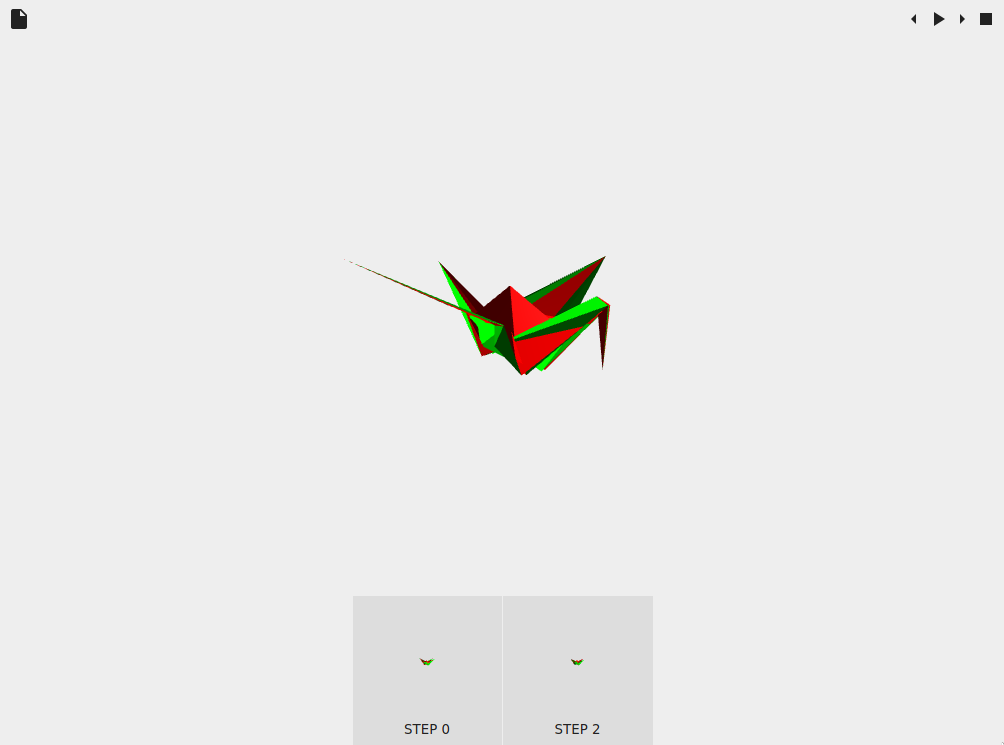
\includegraphics[width=1.01\textwidth]{assets/prototype-front.png}
\end{figure}


% 05-11.04 - FOLD preview prototype
% 12-18.04 - Rewrite in react, file loader, code quality enforcement
% 19-25.04 - Continuous integration setup, lightning changes, solver 
% 24.05-30.05 - Thesis, solver

\subsubsection{May}

During May we refactored the prototype that was developed in April. We adjusted our technology choices and introduced testing libraries.

The most notable aspects that were completed in May include:

\begin{itemize}
	\item first working prototype of the Solver
	\item incorporation of the React framework into the frontend,
	\item the first chapter of the thesis. 
\end{itemize}

\subsubsection{June}

The main topic for May and June was the second chapter of the thesis. The prototype section was written during that time.

\subsubsection{July}

July was not a fruitful month for the project. Several discussions were held, but no actual progress was made.

\subsubsection{August}

In August our focus shifted to performance and stability aspects of the system. 

The most important matters that were wrapped up in August consist of:

\begin{itemize}
	\item adding a damping force to the Solver,
	\item switching the Solver's runtime environment to PyPy,
	\item adding Continuous Integration to the Solver,
	\item supporting target angles in the Solver,
	\item displaying edges with their assignment on the model,
	\item adding timeline scrubbing to the Guide Viewer.
\end{itemize}

\subsubsection{September}

September was a productive time, which brought a lot of business value to the application. 

This time we undertook the implementation of Guide Creator and Community backend parts of the system.
\medskip
We accomplished:

\begin{itemize}
	\item smooth animations with an addition of Guide encoding,
	\item a possibility to compose and create Guides intuitively using the Guide Creator,
\end{itemize}

\subsubsection{October}

In October, we continued working on the community aspect of the system. 

The most valuable features completed in October include:

\begin{itemize}
	\item option to create an account,
	\item ability to log in,
	\item Guide upload functionality,
	\item password reset form,
	\item ability to like a Guide,
	\item Guides Browser,
	\item support for 2D crease patterns.
\end{itemize}


\subsubsection{November}
% 01.11-07.11 - Multi-crease select, triangulation changes, color tweaking,
% 08.11-14.11 - Updating, deleting guides
% 15.11-21.11 - Community backend deployment
% 22.11-now - Thesis, bugfixing

At the beginning of November, we had an application with almost all functional requirements covered. It needed some tweaking, mainly from the User Experience and User Interface points of view. The deadline was nigh. Therefore, we focused all our attention on wrapping up the development process and gaining momentum on writing the paper.

\medskip

We have:

\begin{itemize}
	\item eliminated most of the major pain points from the system,
	\item added Guide deleting and updating functionalities,
	\item widened crease pattern support by changing the triangulation algorithm,
	\item improved visual aspects of the system.
\end{itemize}


\subsubsection{December}

As stated previously, in December we buckled down to writing the thesis and fulfilling formal requirements.
